\section{Umsetzung}

Die App wurde in in XCode 7.2 f"ur iOS9 entwickelt. Zur Umsetzung wurde Swift2 verwendet.  

\subsection{Vorraussetzungen}

Um diese App umsetzen zu k"onnen, mussten zuerst einige Vorraussetzungen erf"ullt werden.

\subsubsection*{API}

Damit diese App realisiert werden konnte musste zuerst eine Verbindung zur API hergestellt werden. 
Diese kommuniziert "uber RESTful Services und ist zu gro"sen Teilen nur "uber eine HTTPS-Verbindung erreichbar. 

Die API kann auf GitHub unter \url{https://github.com/neeedo/neeedo-api} bezogen werden. 
Im Normalfall bietet diese f"ur die lokale Entwicklung eine voll funktionsf"ahige Scala-Applikation die einfach "uber \textit{./sbt
run -Dhttps.port=9443} in einer Konsole gestartet werden kann. Diese ist dann unter \textit{https://localhost:9443/} 

Da Apple in der iOS-Entwicklung nur noch HTTPS-Verbindungen zu zertifizierten Diensten erlaubt, trat hier bereits das erste Problem bei der Umsetzung auf. 
Wenn die API innerhalb der lokalen Entwicklungsumgebung auf \textit{loacalhost} betrieben wird, ist aufgrund von \enquote{Server Trust problems} keine Kommunikation m"oglich.
Dieses Problem lies sich weder durch die Installation eines Zertifikats, noch den Eintrag \enquote{Allow Arbitrary Loads} in der Projektkonfiguration. beheben.

Die L"osung, die am Ende zum Erfolg f"uhrte, war die Installation der API in einem DigitalOcean-Container. Hier war es m"oglich ein Zertifikat zu hinterlegen und eine stabile HTTPS-Verbindung aufzubauen, die eine Kommunikation zwischen API und App erlaubt.

Aktuell l"auft dieser Container noch im Entwicklermodus, und muss manuell gestartet werden. 

\subsubsection*{Konfiguration}

Damit die API korrekt arbeitet m"ussen in der custom-application.conf - File Credentials zu einem Sphere-Shop hinterlegt werden. 
Um bei der Entwicklung vollen Zugriff auf die erstellten Daten zu erhalten, wurde auf  \url{https://admin.sphere.io/} ein neuer Shop angelegt. 
Die n"otigen Daten k"onnen dort unter Entwickler $\rightarrow$ API-Zugriff  gefunden werden.

\subsection{Realisierung}

Bei der Realisierung der dieser App wurde gr"o"stenteils auf den Einsatz von zus"atzlichen Libraries verzichtet, da diese nicht n"otig waren. 

\subsubsection*{Networking}
Die einzige externe Library die in dieser App eingesetzt wurde, ist Alamofire. 

Dies ist eine in Swift geschriebene Networking Library, die Funktionen zur Benutzung von REST-Verbindungen anbietet.
Eine genaue Dokumentation dieser Library kann unter \url{http://cocoadocs.org/docsets/Alamofire/3.2.1/index.html} eingesehen werden.

Der Hauptgrund f"ur die Benutzung dieser Library liegt darin, dass sie den Aufwand bei der Erstellung von HTTP-Requests vereinfacht. 
Sie stellt dabei keine besonderen Zusatzfunktionen bereit, jedoch vereinfacht sie den die Nutzung sehr. (Der ben"otigte Code wird ungef"ahr gedrittelt). 
Dies ist gerade in einem Projekt dass auf sehr vielen solcher Abfragen basiert ein gro"ser Vorteil.

\subsubsection*{Aufbau und Design}

Der Grundlegende Aufbau der App entstand durch den Einsatz in Xcode implementierten Storyboards. 
Hier wurden die ben"otigten Elemente so zusammengesetzt, dass sie die gew"unschten Funktionen erlauben. 

In der aktuellen Fassung wurden das Design beinahe vollst"andig aus Standard-UI-Elemente aufgebaut.
Lediglich einige besondere Custom-Elemente wie Pins wurden zus"atzlich verwedet. 

Wenn die App "uber einen prototypische Entwicklung hinausgeht, k"onnen hier noch ausgestaltete Custom Elemente eingesetzt werden.

Ein durchg"angiges Design wie es in der Android Applikation vorkommt, wurde nicht vollst"andig realisiert, da dies den zeitlichen Rahmen dieser Arbeit gesprengt h"atte. 

\subsection{Wie wurden die Use Cases umgesetzt?}

\subsubsection*{Benutzer}

\begin{figure}[H]
\begin{center}
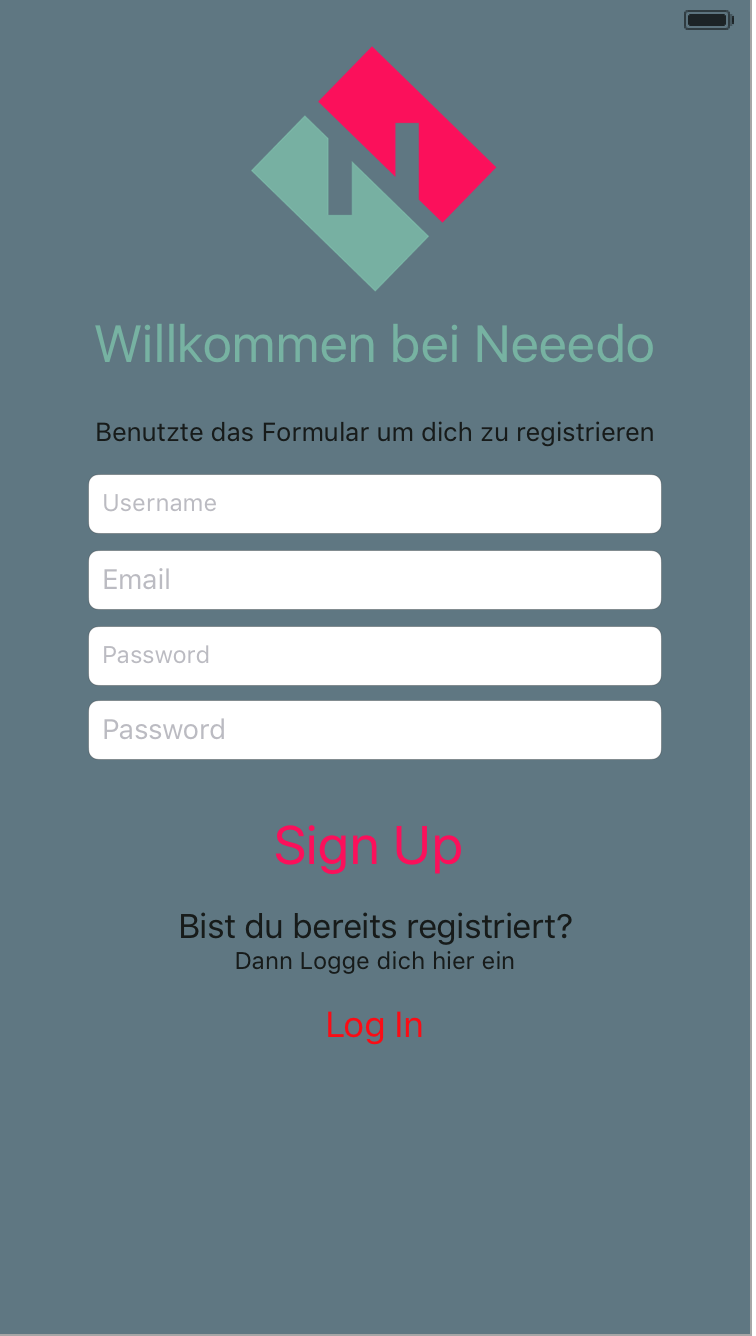
\includegraphics[width=0.45\textwidth]{./Bilder/ioslogin.png}
\caption{SignUpScreen}
\label{fig:ioslogin}
\end{center}
\end{figure}

Wie im Konzept bereits erw"ahnt wurde an der grundlegenden Struktur des Login/SignUps nichts ver"andert. Lediglich farblich wurde es an den rest der Applikation angepasst

\subsubsection{LandingScreen} 

\begin{figure}[H]
\begin{center}
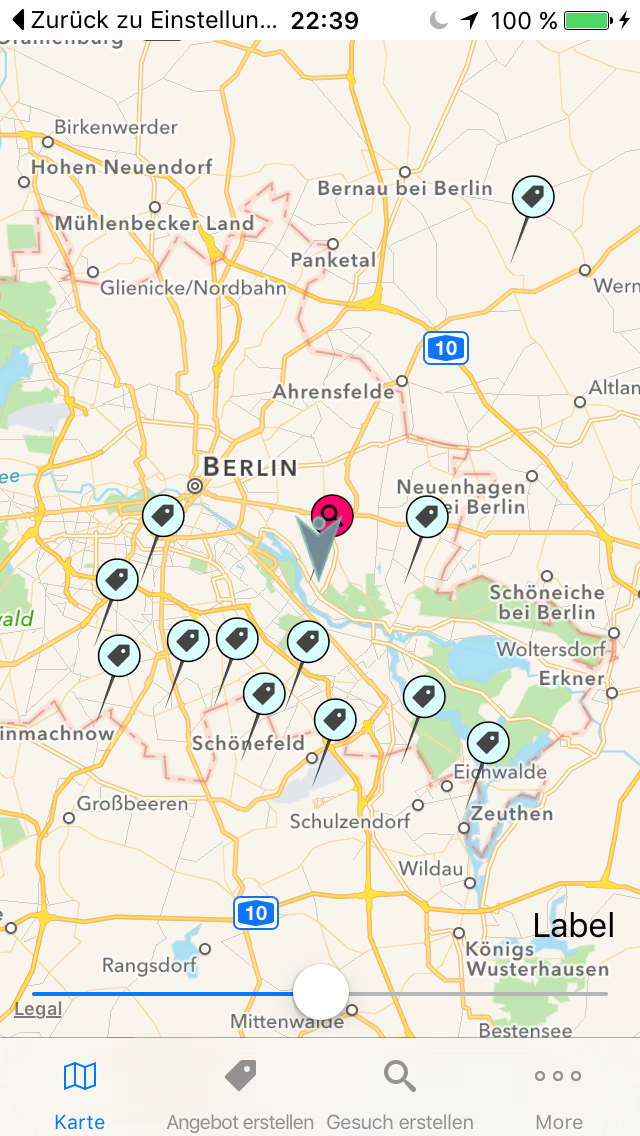
\includegraphics[width=0.45\textwidth]{./Bilder/startscreen.png}
\caption{SignUpScreen}
\label{fig:ioslogin}
\end{center}
\end{figure}

Die gr"o"ste Ver"anderung zur Android App wurde direkt auf dem LandingScreen umgesetzt. Zuvor wurden hier nur zwei  Buttons angezeigt. 
In der neugestalteten Fassung startet man auf einer Karte auf der einem direkt Angebote im Umkreis angezeigt werden. 
Diese Idee wurde so bereits in der WebApp umgesetzt. 

\subsubsection*{Men"u}

\begin{figure}[H]
\begin{center}
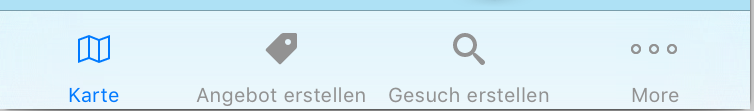
\includegraphics[width=0.45\textwidth]{./Bilder/tabmenu.png}
\caption{SignUpScreen}
\label{fig:ioslogin}
\end{center}
\end{figure}

Diese Ver"anderung des LandingScreens war m"oglich, da man durch die Verlagerung des Men"us in eine Tabbar keinen Bedarf mehr f"ur die beiden zentralen Buttons hatte. 
Das neue Tabbar-Men"u bietet direkten und globalen Zugang zu den wichtigen Erstell-Funktionen, "Uber den Button "Mehr" k"onnen Account spezifische Funktionen wie LogOut, Nachrichten etc. erreicht werden.

\subsubsection*{Angebote, Gesuche erstellen/bearbeiten}

\begin{figure}[H]
\begin{subfigure}{0.5\textwidth}
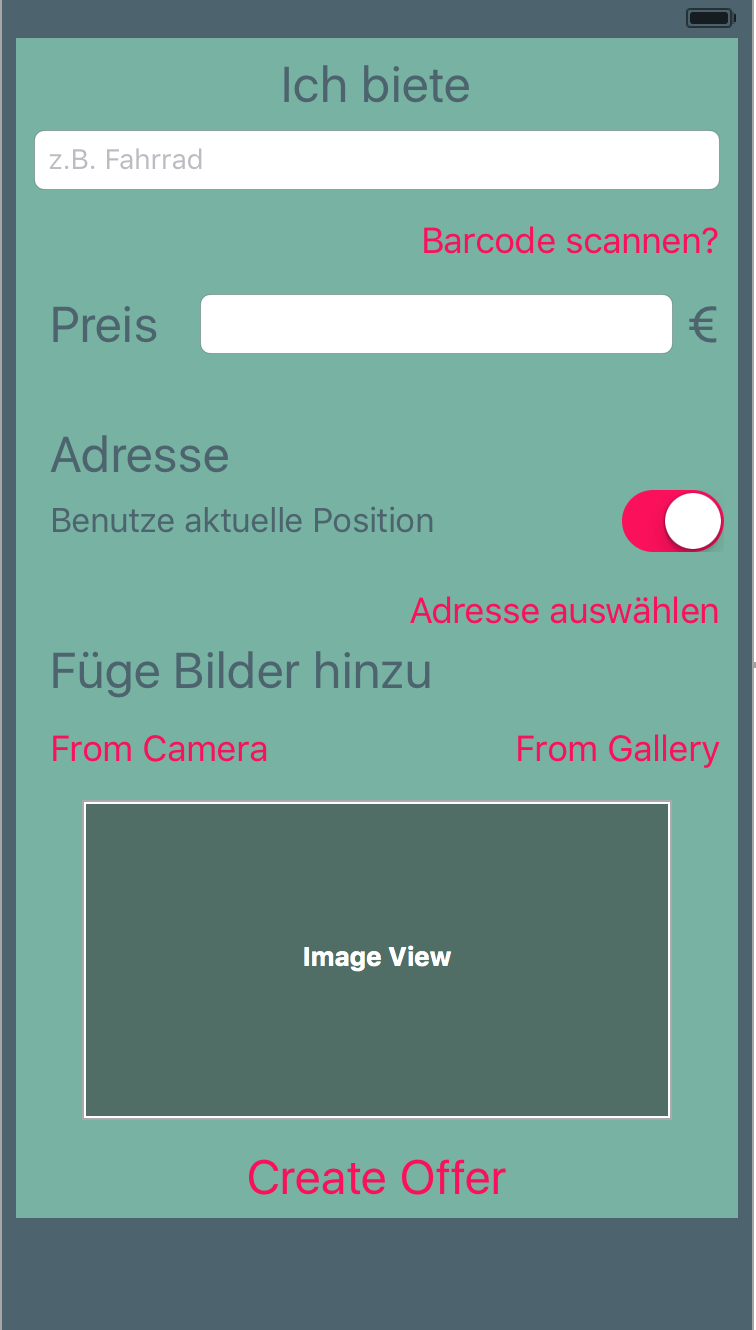
\includegraphics[width=0.9\linewidth]{./Bilder/ioscreateoffer.png} 
\caption{Angebot erstellen}
\label{fig:iosoffer}
\end{subfigure}
\begin{subfigure}{0.5\textwidth}
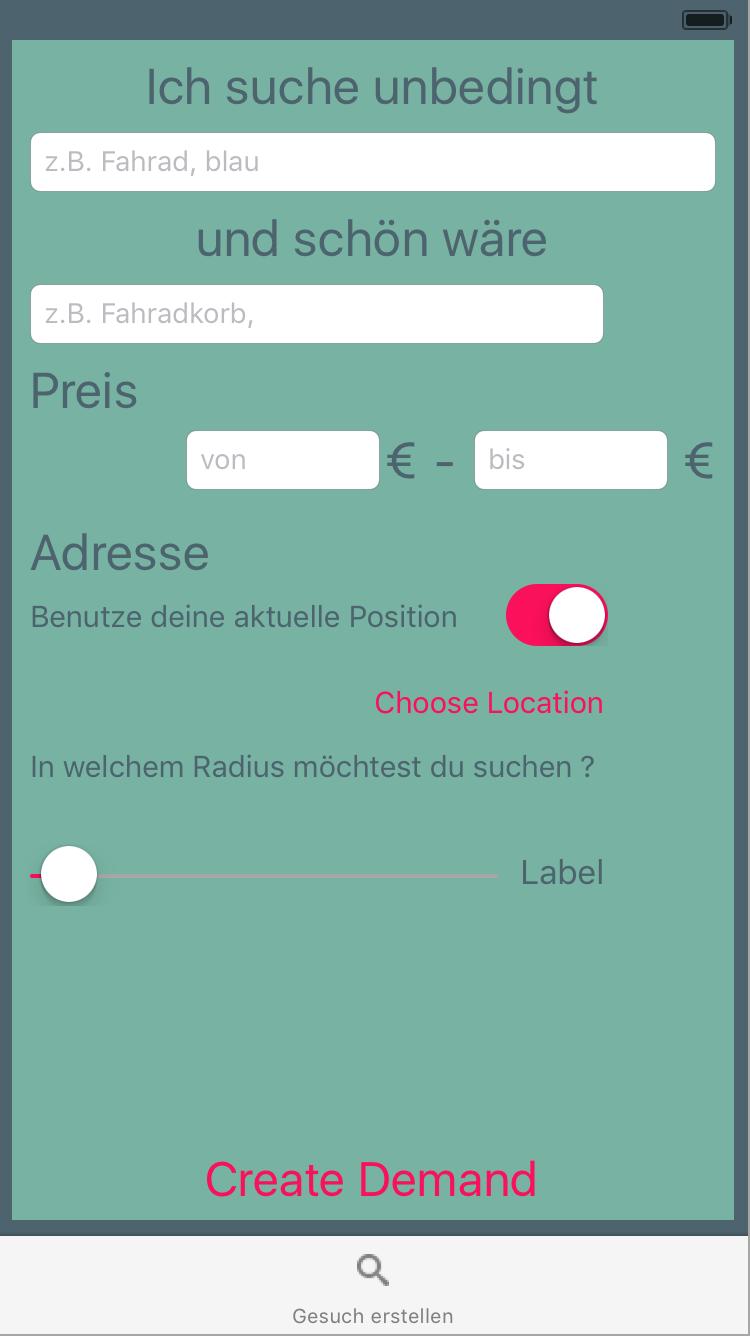
\includegraphics[width=0.9\linewidth]{./Bilder/ioscreatedemand.png}
\caption{Gesuch erstellen}
\label{fig:iosdemand}
\end{subfigure}
\caption{}
\label{fig:image10}
\end{figure}
\subsubsection*{Favoriten}

F"ur das Erstellen und bearbeiten der der Angebote und Gesuche wurde das Konzept der Formulare aus der Android Applikation "ubernommen.
Der gr"o"ste unterschied zur vorherigen Fassung ist das die auswahl der Adresse nicht mehr standardm"a"sig aktiv ist. 
Hier wurde die M"oglichkeit geschaffen direkt zu w"ahlen ob die aktuelle Position genutzt werden soll oder ob man eine andere w"ahlen m"ochte.

Im Formular zum Erstellen eines Angebotes wurden die Funktionen des Barcodescanners, sowie das Hinzuf"ugen von Bildern "ubernommen. 
Der Barcodescanner wurde dabei durch in der AVFoundation-Library zug"angliche Funktionen umgestetzt. 
Die Informationen zu den Codes werden "uber die outpan-API bzogen, die auch in der Android Applikation zum Einsatz kommt. 

Das Hinzuf"ugen von Bildern ist getrennt durch 2 Button dargestellt, um zu verdeutlichen, dass sowohl aus der Gallerie als auch von der Kamera Bilder bezogen werden k"onnen.

\subsubsection*{Matching}

\begin{figure}[H]
\begin{center}
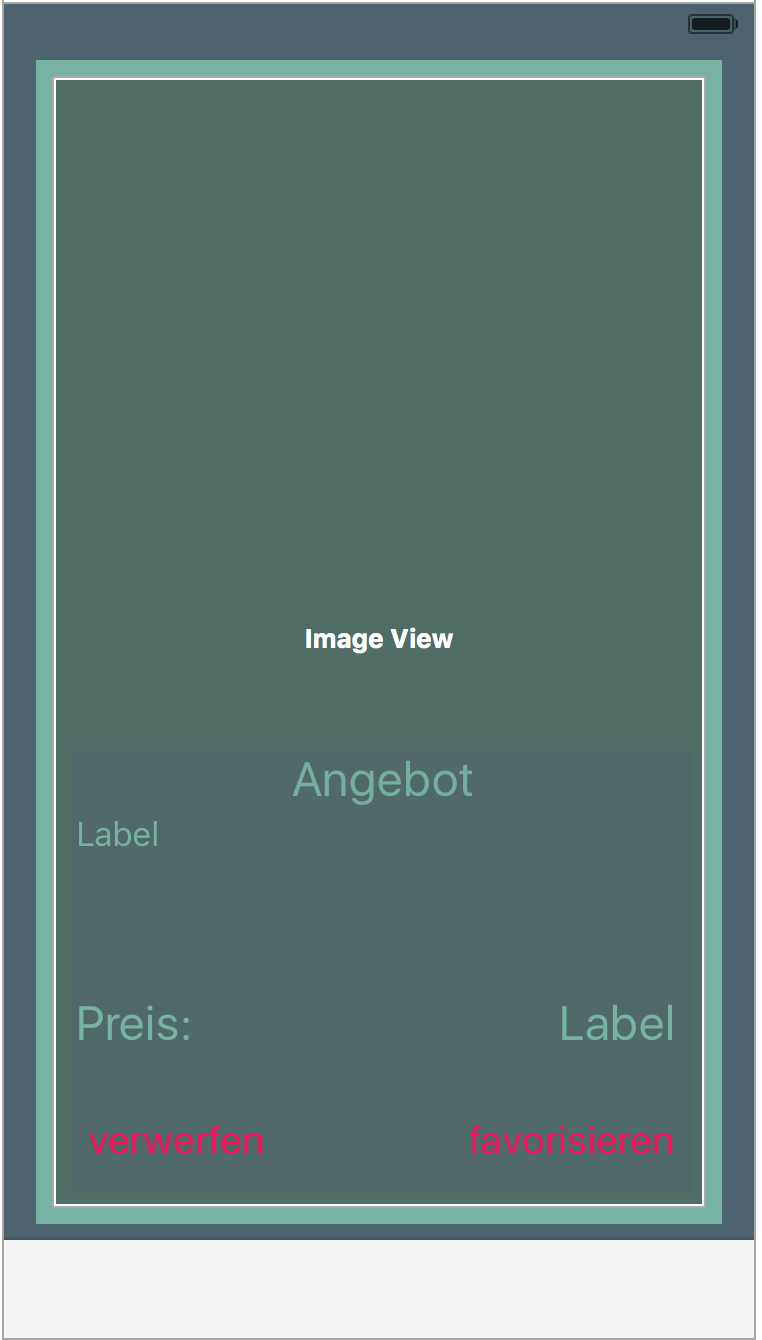
\includegraphics[width=0.45\textwidth]{./Bilder/iosmatch.png}
\caption{SignUpScreen}
\label{fig:ioslogin}
\end{center}
\end{figure}

Das Matching wurde auf ebenfalls durch die Tinder-"ahnliche Swipe ansicht realisiert. Was das Bild hier nicht anzeigt ist, dass das Angebotsbild im Hintergrund angezigt wird, und man die erwarteten Swipe-Gesten nutzen kann. 

\subsubsection*{Favoriten, (Eigene) Angebote, (Eigene) Gesuche anzeigen}

\begin{figure}[H]
\begin{center}
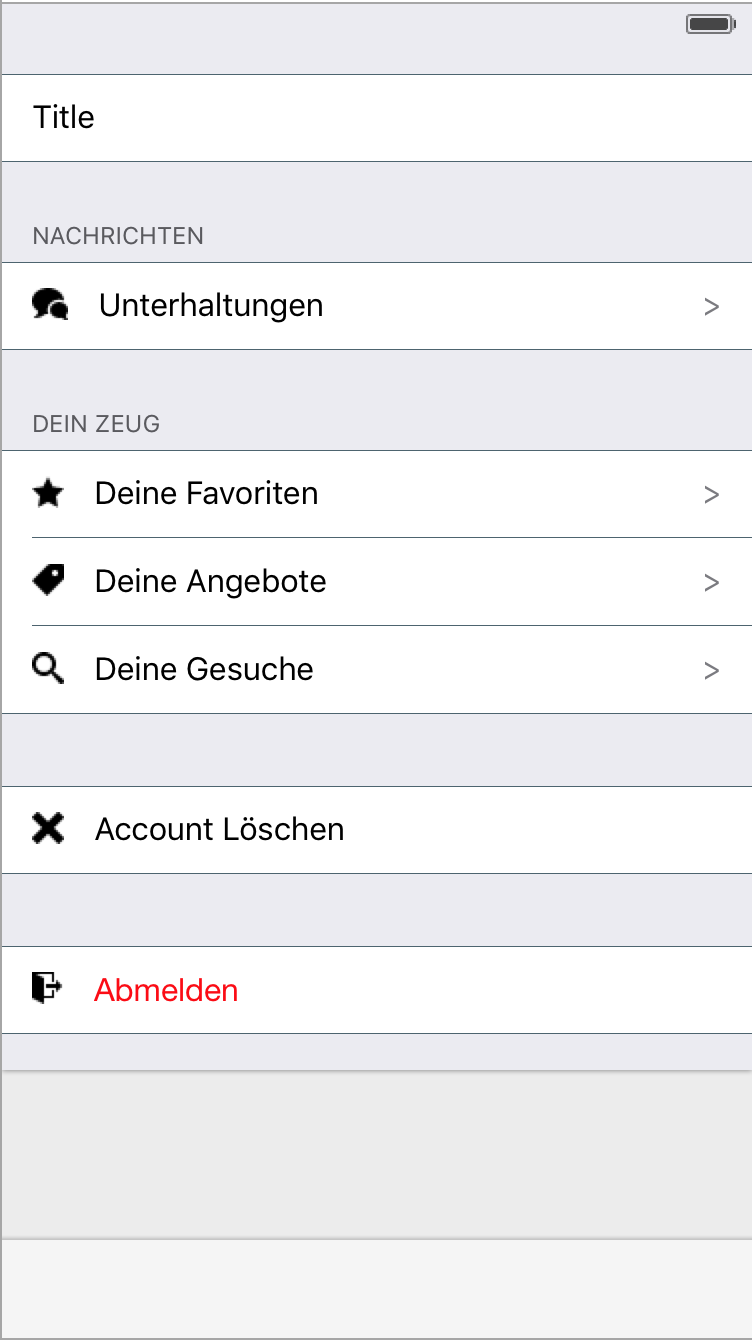
\includegraphics[width=0.45\textwidth]{./Bilder/iosMenu.png}
\caption{SignUpScreen}
\label{fig:ioslogin}
\end{center}
\end{figure}

Die restlichen Funktionalit"aten, die zuvor "uber das Kopf- oder Seitenmen"u  erreichbar waren, wurden zusammengefasst und unter dem Men"upunkt \enquote{Mehr} zug"anglich gemacht.
Hier kann man sich jetzt seine Favoriten, Gesuche und Angebote und Nachrichten anzeigen lassen. Zus"atzlich kann man hier auch seinen Account l"oschen und sich ausloggen.

\subsection{Probleme und L"osungen}

W"ahrend er Entwicklung dieser Applikation traten einige Probleme auf, diese sollen hier einmal mit ihren L"osungen dargestellt werden. 

\subsubsection{Asynchronous Programming}

Ein Problem das bei der Verwendung von RESTful Services h"aufig auftritt, ist das die Antworten(Responses) auf die Anfragen(Requests) oft eine gewisse Zeit in Anspruch nehmen. Damit die App nicht blockiert w"ahrend auf diese Antworten gewartet wird sind die Funktionen die diese Anfragen bearbeiten asynchron aufgebaut. Dies ist so sowohl in Alamofire als auch im klassischen Swift realisiert. 

Anfangs wurde dieser Fakt nicht beachtet, was zu einigen Problemen und Appabst"urzen f"uhrte. 

Die L"osung die hierbei zu verwenden ist, sind sogenannte \textit{Completionhandler} die es erm"oglichen Funktionen abh"angig von der Antwort aufzurufen, d.h. diese werden dann ausgel"ost wenn wirklich eine Antwort vorhanden ist.  

\subsubsection{Kamera}

Das Aufnehmen von Bildern mit der Kamera warf einige Probleme auf, die auch noch nicht behoben sind. Es scheint hier einen h"aufig auftretenden Bug zu geben, der beim Zugriff auf das ungespeicherte Bild auftritt. In diesem Fall erh"alt man den Fehler \enquote{snapshotting a view that has not been rendered results in an empty snapshot. ensure your view has been rendered at least once before snapshotting or snapshot after screen updates.}
Um das zu beheben muss das Bild zwischengespeichert oder angezeigt werden, jedoch scheinen danach in irgendeiner Art Probleme bei der Weiterverarbeitung aufzutreten. 


